\documentclass{standalone}
\usepackage{tikz, graphicx, amsmath, setspace}
%\usepackage{cmbright}
\begin{document}

\begin{tikzpicture}[scale=0.75, every node/.style={scale=0.75}]
{
\setstretch{0.9}
\node [above right] at (0, 0) {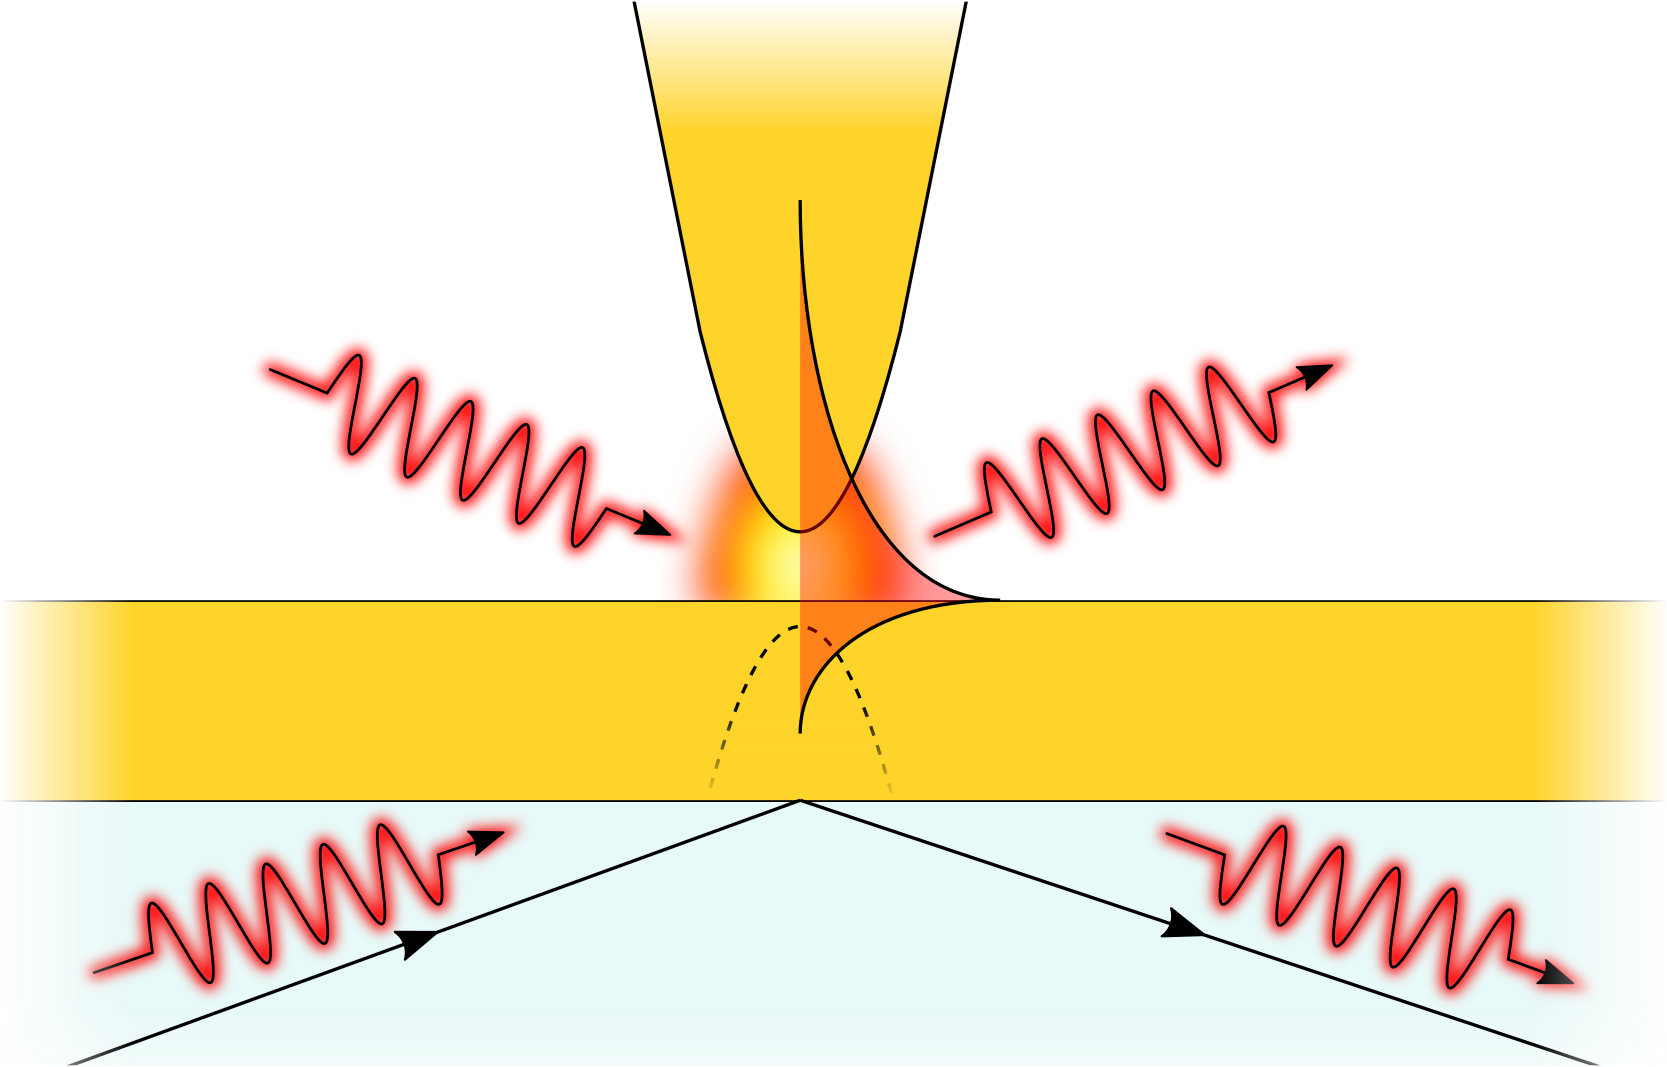
\includegraphics[width=9cm]{tenom_surface.png}};
%\node at (-0.7,5.8) {\textbf{\fontsize{12pt}{1em}\selectfont b}};
\node at (-0.4,5.8) {\textbf{\fontsize{14pt}{1em}\selectfont b}};

%\draw (-0.65,1.85) circle (0.25);
%\node at (-0.65,1.85) {1};
%\draw (-0.35,1.85) circle (0.25);
%\node at (-0.35,1.85) {1};
%\node [align=center] at (4.4,0.8) {evanescent wave\\generation};
%\node [align=center] at (0.15,1.15) {TIR excitation\\$\mathit{NA}>1$};
\node [align=center] at (5.6,2.1) {image\\charge};
\node [align=right] at (2.4,2.25) {hot-spot\\enhanced near-field};

%\draw (0.95,4.2) circle (0.25);
%\node at (0.95,4.2) {2};
%\node at (1.4,4) {$\omega$};
%\node [left] at (10.8,4) {$\omega - \delta\omega$};
%\node [left] at (10.85,3.95) {\bfseries$
%\begin{cases}
%    \omega & \text{a-SNOM}\\
%    \omega - \delta\omega & \text{TERS}
%\end{cases}
%$};

%\draw (7.8,4.9) circle (0.25);
%\node at (7.8,4.9) {3};
%\node [align=left] at (6.25,4.45) {near--far-field\\scattering};

%\draw (9.5,1.8) circle (0.25);
%\node at (9.5,1.8) {4};
%\node [align=center] at (9.25,1.1) {SPP leakage\\radiation};
}

{\fontsize{7pt}{1em}\selectfont \bfseries
\color{blue}
\node at (4.2,3.55) {$-$};
\node at (4.45,3.2) {$-$};
\node at (4.7,3.55) {$-$};
\node at (4.2,2.55) {$-$};
\node at (4.7,2.55) {$-$};
\color{red}
\node at (4.3,3.35) {$+$};
\node at (4.6,3.35) {$+$};
\node at (3.95,2.55) {$+$};
\node at (4.45,2.55) {$+$};
\node at (4.95,2.55) {$+$};
}

\end{tikzpicture}

\end{document}